\section{Sensitivity Analysis}

\subsection{Model 1}
Model 1 is an AHP-based method network, which has two parameters:
\begin{itemize}
\item \textbf{Parameter 1:} Weight matrix
\item \textbf{Parameter 2:} Plan weight matrix
\end{itemize}

Changes in both parameters can affect the final result, but the weight matrix has a greater impact. For each plan, its requirement for the weight matrix is usually fixed. For example, the requirement for Sustainable Development Goal 1: No Poverty is fixed, and we have calculated that the Importance weight for Goal 1 is the largest, at 0.302. These data are related to the nature of each SDG and are generally fixed. 
\begin{figure}[h]%插入图片并且加上图片的标题,这是一个模板
    \centering
    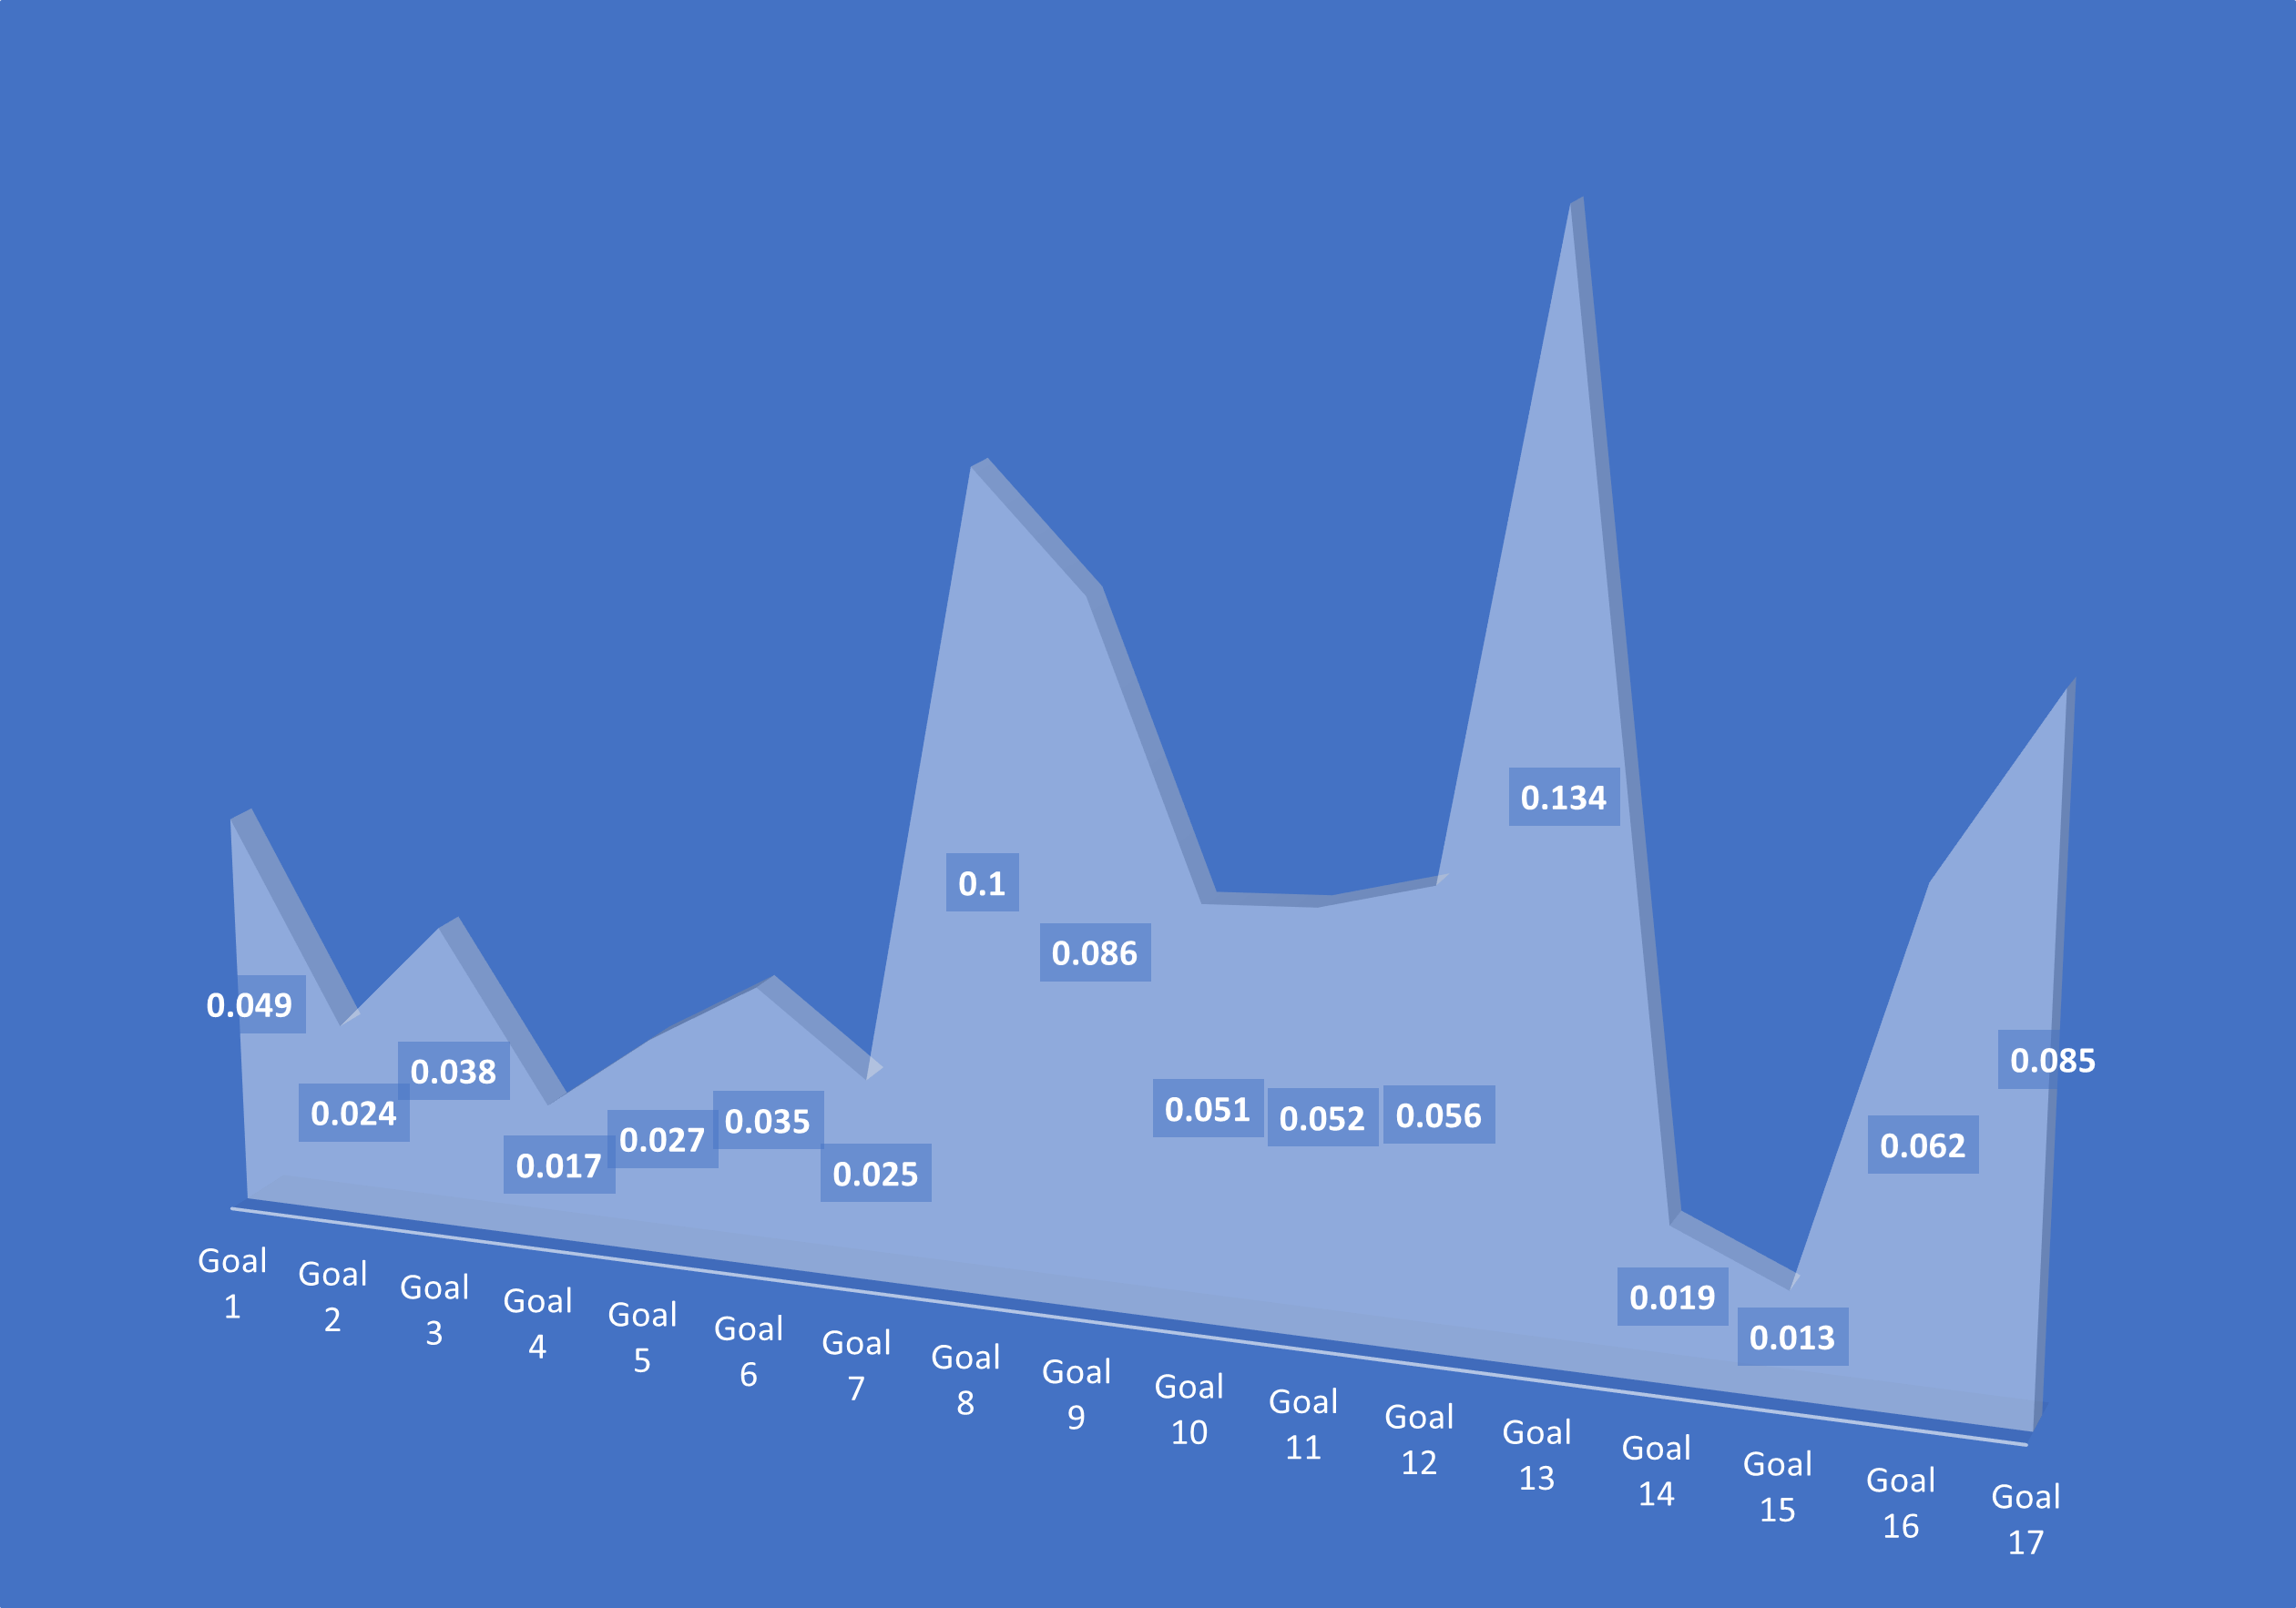
\includegraphics[scale=0.45]{{figure/Sen-1.png}}%插入图片的指令
    \caption{Weight of changes after minor perturbations}%标题
    \label{Label}
\end{figure}
They may vary slightly in different countries or regions, but this is not within the scope of our consideration. 
The impact of the weight matrix is significant, especially for Model 1, which requires 17 plans to be changed through the assignment of weight matrix values. 

If we change the parameters of the weight matrix.then the 17 plans would change as above.
Therefore, slight changes in the weight matrix have high sensitivity in Model 1 and can lead to many changes in the final results.

\subsection{Model 2 and Model 3}
\textbf{Model 2} is based on K-means and AHP, and has three parameters:
\begin{itemize}
\item \textbf{Parameter 1:} Weight Matrix
\item \textbf{Parameter 2:} Solution Weight Matrix
\item \textbf{Parameter 3:} Number of Clusters in K-Means
\end{itemize}

The result of K-means clustering directly affects the calculation of AHP weights, so the size of K will have a significant impact on the final result. We can try changing the value of K and observe the change in SDG weights.

In the AHP method, the composition of the decision layer and the criterion layer will also affect the final weights. We can try changing the composition of the decision layer or criterion layer and observe the change in SDG weights. This is similar to the sensitivity analysis in Model 1.

Task 2 requires us to consider the \textbf{scalability and development} of our model when a certain indicator is achieved. This actually involves changing the types and weight matrices of solutions. K-means clustering will introduce some changes, and AHP weights will also change. Among them, the weight matrix is still the most important. Similar to Model 1, when hunger is completely eliminated, the individual properties of different sustainable development goals will differ, thereby affecting the allocation of weights.\\

\textbf{Model 3} is an \textbf{optimized version} of Model 2, based on K-means and AHP. The parameter settings are the same as in Model 2, but the weight module has been changed to use the 5Ps for weight analysis. The most important parameter in this part is undoubtedly the changes in the weight of the 5Ps, as Model 3 is aimed at solving the requirements of task 4, which involves addressing the demand situation in the event of global climate change. We made tentative changes to the weight of the 5Ps, and the overall data changes are shown in the figure below:

\begin{figure}[h]
\centering
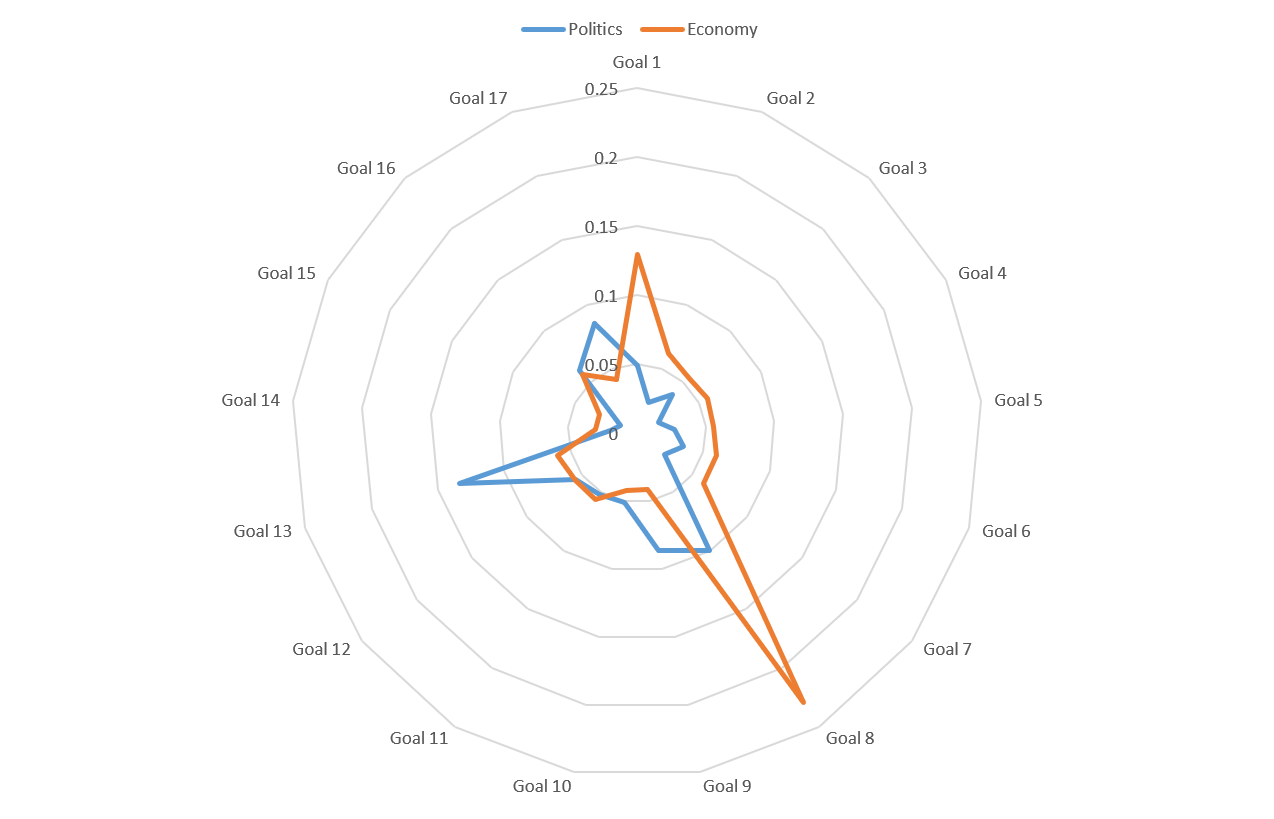
\includegraphics[scale=0.65]{{figure/Politics&Economy.png}}
\caption{Weight of changes after minor perturbations}
\label{Label}
\end{figure}

Our changes to the weight of the 5Ps demonstrate the impact of changes in global events on our model or the changes in weight that may occur due to the evolving global situation. By adjusting the weights of the 5Ps, our model can effectively adapt to changes in global priorities and shifting focus on specific goals, making it a robust tool for sustainable development planning and decision-making. The flexibility and adaptability of our model make it a valuable asset for policymakers and stakeholders to assess and evaluate the progress of the SDGs and make informed decisions accordingly.

In addition, the model provides valuable insights for decision-makers to design effective policies and strategies to achieve sustainable development goals in different countries and regions. It also serves as a useful reference for future research on sustainable development and decision-making, providing a systematic and quantitative approach to address complex global issues. Overall, our model has the potential to make a significant contribution to promoting sustainable development and achieving a better future for all.




